% !TeX root = ../bbchallenge-paper.tex
\newpage
\subsection{Loops}\label{sec:loops}
\subsubsection{Algorithm}\label{sec:loops:algo}

\begin{figure}[h!]
    \centering
    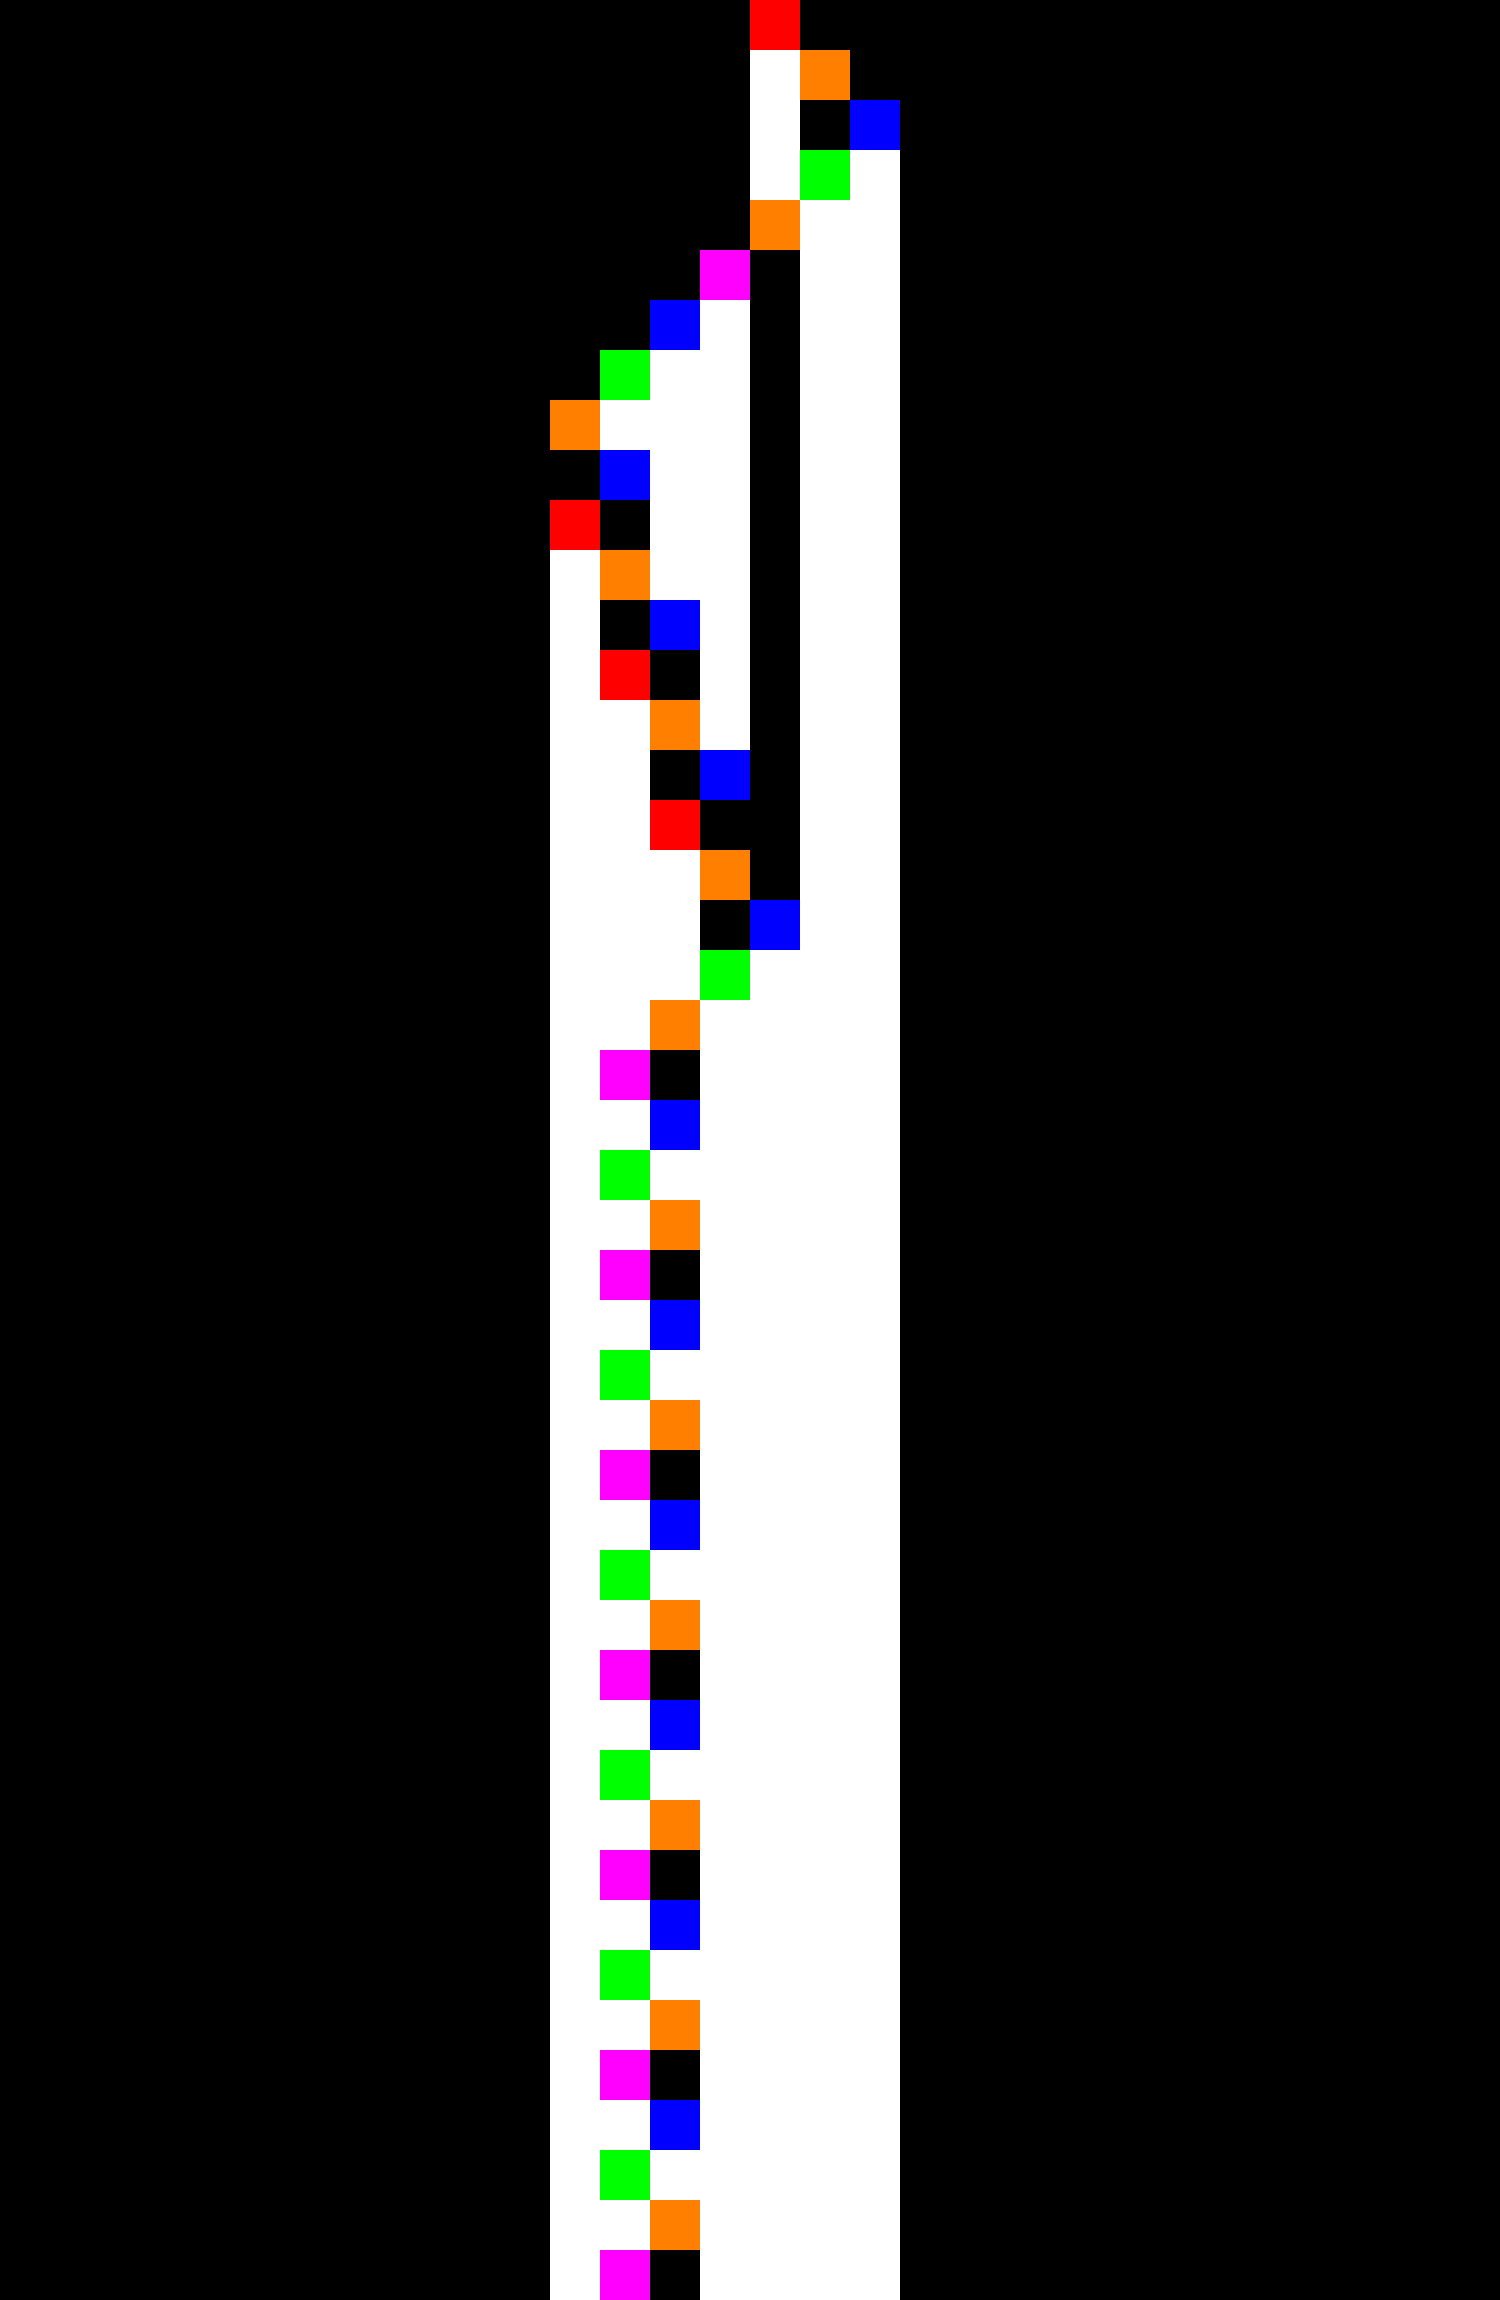
\includegraphics[width=0.28\textwidth]{figures/space-time-diagrams/cycler_279081.pdf}
    \hspace{10ex}
    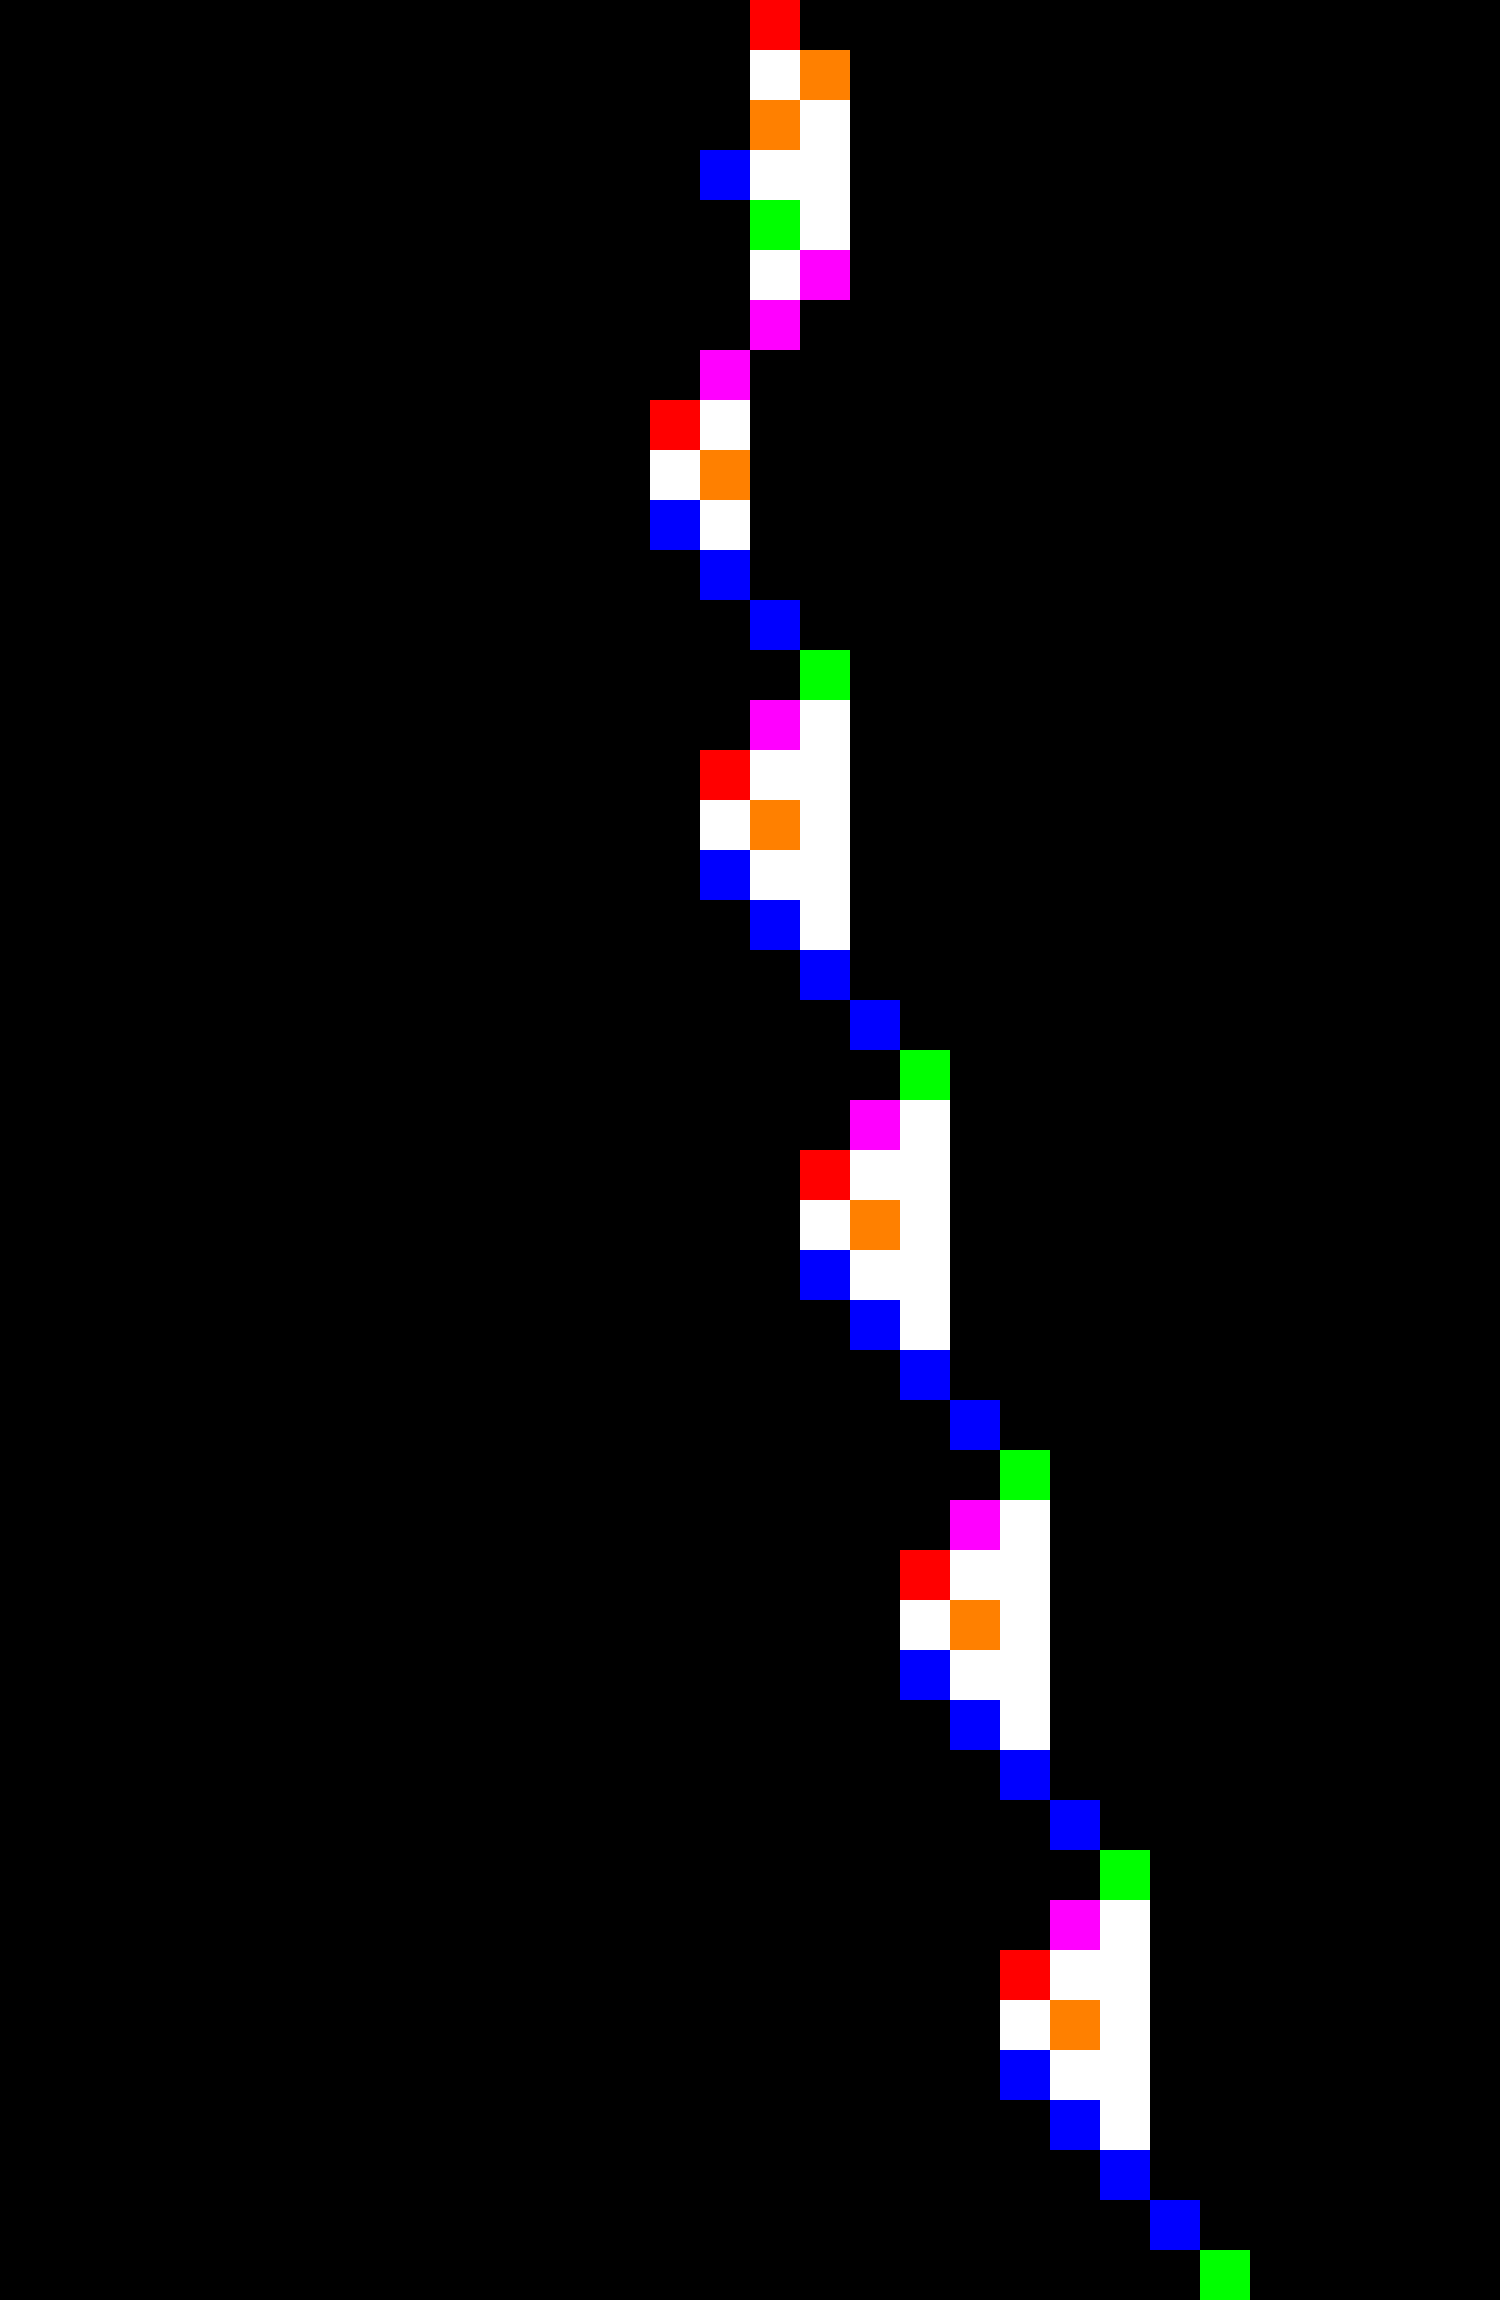
\includegraphics[width=0.28\textwidth]{figures/space-time-diagrams/tc_1RB---_1LB1LC_0RD0RC_1LE1RE_1LA0LE.pdf}
    %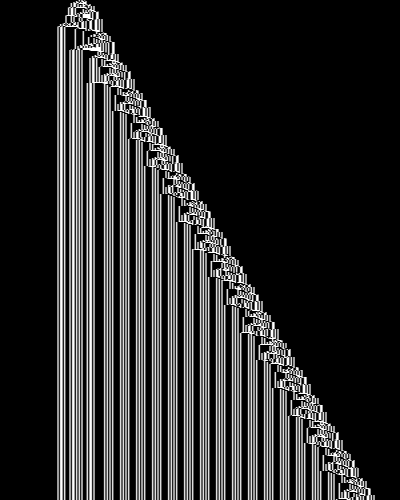
\includegraphics[width=0.4\textwidth]{figures/space-time-diagrams/translated_cycler_59090563_2.png}
    \caption{Space-time diagrams of the 30 first steps of a \textit{\cycler}, \href{https://bbchallenge.org/1RB---\_0RC0LE\_1LD0LA\_1LB1RB\_1LC1RC}{\texttt{1RB---\_0RC0LE\_1LD0LA\_1LB1RB\_1LC1RC}} (left) and of the 10,000 first steps of a \textit{\TC}, \href{https://bbchallenge.org/1RB---\_1LB1LC\_0RD0RC\_1LE1RE\_1LA0LE}{\texttt{1RB---\_1LB1LC\_0RD0RC\_1LE1RE\_1LA0LE}} (right). \cyclers are machines that eventually repeat the same configuration forever. \TCs are machines that eventually repeats the same configuration forever, but translated in space. We refer to these two types of machines as \textit{loops}.}\label{fig:loops}
\end{figure}

% \footnotetext{\url{https://bbchallenge.org/1RB---\_0RC0LE\_1LD0LA\_1LB1RB\_1LC1RC}}
% \footnotetext{\url{https://bbchallenge.org/1RB---\_1LB1LC\_0RD0RC\_1LE1RE\_1LA0LE}}

The goal of this decider is to recognise two types of Turing machines: (i) \textit{\cyclers} (see Figure~\ref{fig:loops}~left) that eventually repeat the same configuration and therefore loop forever and (ii) \textit{\TCs} that also eventually repeat the same configuration, but translated in space (see Figure~\ref{fig:loops}~right), analogous to \textit{gliders} in cellular automata. We regroup both types of machines under the umbrella term of \textit{loops}.

Deciding Cyclers reduces to the well-known mathematical problem of detecting the cycles of a function and standard detection algorithms exist \cite{wiki:Cycle_detection}, the simplest one consisting in memorizing each successive configuration of the machine until encountering one that has been already seen. Translated Cyclers, also known as \textit{Lin's recurrence}, have first been described and decided in Shen Lin's 1963 PhD thesis \cite{Lin1963}, other similar algorithms to detect them have been developed since then\footnote{\url{https://discuss.bbchallenge.org/t/decider-translated-cyclers/34}}.

Here, we develop a completely different algorithm (Algorithm~\ref{alg:loops}) for deciding both \cyclers and \TCs at once. The particularity of this algorithm is that it detects loops only by analysing the history of state, read-symbol and \headposs visited by the machine, instead of considering entire configurations (\ie with full tape content information). Hence, in theory, Algorithm~\ref{alg:loops} can be implemented to use less memory than previously-known algorithms\footnote{In practice, for simplicity, the Coq implementation stores entire tapes (whereas it only uses the head's information), hence it does not avail of this potential memory optimisation.}.

Let's call the \textit{transcript} of a machine the list of successive \ssps visited by the machine from the all-zero tape. For instance, the transcript of the \cycler in Figure~\ref{fig:loops}~(left) starts with \texttt{A0 B0 C0 D0 B1 E0 C0 D0 B0 C1 A0} and the transcript of the \TC in Figure~\ref{fig:loops}~(right) starts with \texttt{A0 B0 C0 A0 B1 D1 C1 E0 C0 A1 C1}. Surprisingly, it turns out that in order to detect loops, we only have to track when a transcript repeats the same sequence twice back-to-back, for instance, in the case of the Cycler in Figure~\ref{fig:loops}: \texttt{A0 B0 C0 D0 B1 E0 C0 D0 B0 C1 A0 B0 C1 A0 B0 C1 A0 B0 C0 D0 \textbf{\underline{B1 E1 C0 D1}} \textbf{\underline{B1 E1 C0 D1}}}. When such a repetition occurs, we use the extra information of \headpos to conclude:

\begin{enumerate}
    \item If when entering the second repetition the head is at the same position it was at the beginning of the first repetition, then we have detected a \cycler, \eg for the \cycler in Figure~\ref{fig:loops}~(left), here is the end of the transcript with extra head-position information given after each \ssp: \texttt{\underline{\textbf{B1(-2)} E1(-3) C0(-2) D1(-3)} \underline{\textbf{B1(-2)} E1(-3) C0(-2) D1(-3)}}.
          %This case is covered by Theorem~\ref{th:loops:theory}, Case 1.

    \item If, at the beginning of both repetitions, the head is at the same extremity of the tape (\ie both positions are either both a local maximum or both a local minimum) then we have detected a \TC. For the \TC in Figure~\ref{fig:loops}~(right):  \texttt{A0(0)* B0(1)* B1(0) C0(-1) D1(0) E1(1)* E1(0) E0(-1) A0(-2) B1(-1) C1(-2) C1(-1) C0(0) \\  \underline{\textbf{D0(1)* E0(0) A0(-1) B1(0) C1(-1) C1(0) C1(1)* C0(2)*}} \\ \underline{\textbf{D0(3)* E0(2) A0(1) B1(2) C1(1) C1(2) C1(3)* C0(4)*}}} where \texttt{*} indicates steps where the machine is at the right-extremity of the tape (\headpos local maximum).


\end{enumerate}

We prove that Algorithm~\ref{alg:loops} is correct in Theorem~\ref{th:loops}.




\begin{algorithm}
    \caption{{\sc decider-Loops}, reformulates the algorithm \texttt{loop1\_decider} of Coq-BB5.}\label{alg:loops}

    \begin{algorithmic}[1]
        \State{\textbf{Input:} A Turing machine `$\mathcal{M}$', a step-limit parameter $L$.}
        \State{\textbf{Output:} \NONHALT if the decider detects that the machine is a loop, \HALT if the machine halts and \UNKNOWN otherwise.}

        \State
        \State Simulate $\mathcal{M}$ for $L$ steps and save the history of each consecutive state, read-symbol and position, \ie consecutive $T_i = (s_i,m_i,d_i)\in\states\times\alphabet\times\Z$ for $0 \leq i \leq L$ and $T_0 = (\stateA,\symbolzero,0)$.


        \State \If{the machine has halted before $L$ steps}
        \State \Return HALT \label{alg:loops:halt}
        \EndIf
        \State \For{$l$ \textbf{in} $[1,+\infty[$ } \Comment{$l$ is the length of the potential loop}
        \State \If{$2l > L$} \Comment{The history does not contain two transcript repetitions of size $l$}
        \State \Return UNKNOWN \label{alg:loops:terminate}
        \State \EndIf
        \State $K = L-l-1$
        \State $o = 0$ \Comment{Offset in case we need to keep looking for local-extremum}
        \State $\text{allequal} = \text{true}$
        \State \For{$i$ \textbf{in} $[0,l+o[$ }
        \If{$K-i < 0$}
        \State \textbf{break}
        \State \EndIf
        \State $s,m,d = T_{L-i}$
        \State $s',m',d' = T_{K-i}$
        \State
        \If{$s\neq s'$ \textbf{or} $m \neq m'$}\label{alg:loops:testeq} \Comment{Comparing \ssp equality at each step}
        \State \textbf{break}
        \EndIf

        \State \If{$i = l+o-1$}
        \If{$d = d'$}\label{alg:loops:cycler}
        \State \Return \NONHALT \Comment{We've detected a Cycler}
        \EndIf
        \State \If{$d = \text{max} \{d_j \, | \, j < L-i \}$ \textbf{and} $d' = \text{max} \{d_j \, | \, j < K-i \}$}\label{alg:loops:tcplus}
        \State \Return \NONHALT \Comment{We've detected a (positive) Translated Cycler}
        \EndIf
        \State \If{$d = \text{min} \{d_j \, | \, j < L-i \}$ \textbf{and} $d' = \text{min} \{d_j \, | \, j < K-i \}$}\label{alg:loops:tcminus}
        \State \Return \NONHALT \Comment{We've detected a (negative) Translated Cycler}
        \State \EndIf
        \State $o = o + 1$
        \State \EndIf
        \EndFor
        \EndFor

        \State \Return \UNKNOWN

    \end{algorithmic}

\end{algorithm}


\subsubsection{Correctness}
Proving the correctness of this decider is surprisingly nontrivial. Let's represent the space-time diagram of a given Turing machine $\mathcal{M}$ (Section~\ref{sec:TMs}) using partially defined functions $f_\mathcal{M},g_\mathcal{M},h_\mathcal{M}$:
\begin{align*}
    f_\mathcal{M} & : \N \hookrightarrow \Z \to \alphabet\text{, tape content}                                \\
    g_\mathcal{M} & : \N \hookrightarrow \Z\text{, head position}                                             \\
    h_\mathcal{M} & : \N \hookrightarrow \states\text{, head state}                                           \\
    F_\mathcal{M} & : \N \hookrightarrow \Z \to (\alphabet\times \states)\text{, tape content and head state}
\end{align*}

\newcommand{\baref}{F}

At time $t\in\N$, $f_\mathcal{M}(t)$ gives the tape content (as a total function $\Z \to \alphabet$), $g_\mathcal{M}(t)$ gives the head position and $h_\mathcal{M}(t)$, the head state, assuming in each case that $\mathcal{M}$ has not halted before time $t$, otherwise values are not defined. For brevity, when the Turing machine is clear from context, we may write $f,g,h$. In the case of $f$, we will also use notation $f(t,z)$ or $f(p)$ with $p \in \N \times \Z$ seen as a vector, instead of $f(t)(z)$ when $f(t)$ is defined. Using same extended notations as for $f$, we also define $\baref_\mathcal{M}(t,z) = (f(t,z),h(t))$ which gives tape content with head state information at each time when $f$ and $h$ are defined.
Finally, when assuming/claiming $f(x) = f(y)$ for some $x,y \in \N \times \Z$ we also implicitly assume/claim that $f$ is defined at $x$ and $y$; same for $\baref$, $g$, and, $h$.

Transcripts as defined in Section~\ref{sec:loops:algo} correspond to sequences of the form $F_\mathcal{M}(t,g(t))$ with $t\in\N$.

\begin{figure}[h!]
    \noindent
    \begin{minipage}[t]{1\textwidth}
        \centering
        \scalebox{0.85}{
            \begin{tikzpicture}[every node/.style={minimum size=6mm, draw, font=\scriptsize}, scale=1]

                \draw[->, thick] (-1.3,2.7) -- (-1.3,1.7) node[draw=none, midway, left] {\scriptsize time};
                \draw[->, thick] (-1.3,2.7) -- (-0.3,2.7) node[draw=none, midway, above] {\scriptsize space};










                % \node[draw=none] at (-1,2.7) {$p_0$};
                % \draw[-{Latex[length=1.8mm]}] (-0.8,2.6) -- (-0.4,2.3);
                \node (C1) at (0,2) {\stateCx\sone};
                \node[draw=black, draw opacity=0.6] (A1) at (0.6,1.4) {\stateAx\sone};
                \node[draw=black, draw opacity=0.6] (B0) at (1.2,0.8) {\stateEx\szero};
                \node[draw=black, draw opacity=0.6] (D0) at (0.6,0.2) {\stateDx\szero};

                % % Fill 5 cells to the right of C1
                % \foreach \i in {1,...,4} {
                %         \node[minimum size=6mm, draw=none, fill=gray!20] at ($(C1)+(0.6*\i,0)$) {};
                %     }



                \node[dashed, draw=red, thick] (red) at (1.2,0.8) {};

                \node (C1') at (1.2, -0.4) {\stateCx\sone};
                \node[draw=black, draw opacity=0.6] (A1') at (1.8, -1.0) {\stateAx\sone};
                \node[draw=black, draw opacity=0.6] (B0') at (2.4, -1.6) {\stateEx\szero};
                \node[draw=black, draw opacity=0.6] (D0') at (1.8, -2.2) {\stateDx\szero};

                % % Fill 5 cells to the right of C1'
                % \foreach \i in {1,...,4} {
                %         \node[minimum size=6mm, draw=none, fill=gray!20] at ($(C1')+(0.6*\i,0)$) {};
                %     }

                \node[dashed, draw=red, thick] (red') at (2.4,-1.6) {};

                \node[dashed] (C1'') at (2.4,-2.8) {\stateCx?};

                \draw[dashed, draw=red, thick, ->, >=stealth] (red.south) -- (C1'.north);
                \draw[dashed, draw=red, thick, ->, >=stealth] (red'.south) -- (C1''.north);

                % \node[draw=none] at ($(red.north east)+(0.6,0.3)+(0.2,0.05)$) {$\overline{p_0}$};
                % \draw[-{Latex[length=1.8mm]}] ($(red.north east)+(0.6,0.3)$) -- ($(red.north east)-(-0.05,0.00)$);

                % \node[draw=none] at ($(red'.north east)+(0.6,0.3)+(0.2,0.05)$) {$\overline{p_0'}$};
                % \draw[-{Latex[length=1.8mm]}] ($(red'.north east)+(0.6,0.3)$) -- ($(red'.north east)-(-0.05,0.00)$);

                % Arrow and label for p_1
                \node[draw=none] at ($(C1.north east)+(0.6,0.3)+(0.2,0.05)$) {$p_0$};
                \draw[-{Latex[length=1.8mm]}] ($(C1.north east)+(0.6,0.3)$) -- ($(C1.north east)-(-0.05,0.00)$);

                \node[draw=none] at ($(C1'.north east)+(0.6,0.3)+(0.2,0.05)$) {$p_0'$};
                \draw[-{Latex[length=1.8mm]}] ($(C1'.north east)+(0.6,0.3)$) -- ($(C1'.north east)-(-0.05,0.00)$);

                \node[draw=none] at ($(C1''.north east)+(0.6,0.3)+(0.2,0.05)$) {$p^*$};
                \draw[-{Latex[length=1.8mm]}] ($(C1''.north east)+(0.6,0.3)$) -- ($(C1''.north east)-(-0.05,0.00)$);

                \node[draw=none] at ($(B0'.north east)+(0.6,0.3)+(0.2,0.05)$) {$p'_k$};
                \draw[-{Latex[length=1.8mm]}] ($(B0'.north east)+(0.6,0.3)$) -- ($(B0'.north east)-(-0.05,0.00)$);

                \node[draw=none] at ($(B0.north east)+(0.6,0.3)+(0.2,0.05)$) {$p_k$};
                \draw[-{Latex[length=1.8mm]}] ($(B0.north east)+(0.6,0.3)$) -- ($(B0.north east)-(-0.05,0.00)$);

            \end{tikzpicture}
        }
    \end{minipage}
    \caption{Illustration of Lemma~\ref{lem:vector}: head-only space-time diagram showing transcript repetition \texttt{\textbf{\underline{C1 A1 E0 D0}} \textbf{\underline{C1 A1 E0 D0}}}. Coordinates $p_0 = (t_0,g(t_0))$ correspond to the beginning of the first repetition, and $p'_0 = (t_0',g(t_0'))$ of the second. At position $p^*$, we can easily show that the machine shares same state, \stateC, than at position $p_0'$, Lemma~\ref{lem:vector}~Point~\ref{lem:vector:pt2}. Less immediate, in this case, using $p_k$ and $p'_k$, we can show that positions $p^*$ and $p_0'$ also share same read-symbol (depicted as \texttt{?} to signify that it is less immediate to show), which is the symbol outputted after $p_k$ and $p_k'$, Lemma~\ref{lem:vector}~Point~\ref{lem:vector:pt4}. }\label{fig:loop-lemma}
\end{figure}


\begin{lemma}\label{lem:vector} Let $\mathcal{M}$ be a Turing machine.
    Assume there is $ t_0 \in \N$ and $l \in \N^+$ such that
    for all $0 \leq i < l$: $$F_\mathcal{M}(p_i)   = F_\mathcal{M}(p'_i)$$

    with $t_i = t_0 + i$, $t_i' = t_i+l$ and $p_i = (t_i, g(t_i))$, $p_i' = (t_i', g(t_i'))$. Call $p^*=(t^*,g(t^*))$ with $t^*=t'_0 + l$. Then:
    \begin{enumerate}
        \item For all $0 \leq i < l$ we have: $p'_i - p_i = p_0' - p_0$. We also have $p^* - p_0' = p_0' - p_0$. \label{lem:vector:pt1}
        \item We have $h(t^*) = h(t'_0)$.\label{lem:vector:pt2}
        \item For all  $0 \leq i < l$, $g(t_i) = g(t_0') \Leftrightarrow g(t_i') = g(t)$.\label{lem:vector:pt3}
        \item If there is $0 \leq k < l$ such that $g(t_k') = g(t^*)$ then $f(p^*) = f(p_0')$.\label{lem:vector:pt4}
    \end{enumerate}
    Figure~\ref{fig:loop-lemma} illustrates this Lemma and Point~\ref{lem:vector:pt4} in particular.
\end{lemma}
\begin{proof}
    First note that by definition, all $p_i$ and $p_i'$ correspond to head positions and the condition $F_\mathcal{M}(p_i)   = F_\mathcal{M}(p'_i)$ means that there is a repetition in the machine's transcript (see Section~\ref{sec:loops:algo}).
    \begin{enumerate}
        \item Because $F(p_0) = F(p'_0)$ we know that at times $t_0$ and $t_0'$ the head is in same state, reading the same symbol, hence the same transition executes and, in particular, both heads move in the same direction $m \in \{-1,1\}$, giving the existence of $u = (1, m)$ such that $p_1 = p_0 + u$ and $p_1' = p_0' + u$. Hence, $p_1' - p_1 = p_0' + u - p_0 + u = p_0' - p_0$. Repeating the same argument for each $i < l$ gives $p_i' - p_i = p_0' - p_0$. Finally, applying the same argument with $F(p_{l-1}) = F(p'_{l-1})$ gives $p^*-p_0' = p'_0 - p_0$ as $p^*$ corresponds to one time step after $p'_{l-1}$ and $p'_0$ one time step after $p_{l-1}$.
        \item Similarly to above, $F(p_{l-1}) = F(p'_{l-1})$ implies that the machine will transition to the same state after $p_{l-1}$ and $p'_{l-1}$, giving $h(t^*) = h(t')$.

        \item Let $0 \leq i < l$ such that $g(t_i) = g(t_0')$. Using Point~\ref{lem:vector:pt1}, we have $p_i' = p_i + (p_0' - p_0)$, meaning $g(t_i) = g(t_0') \Leftrightarrow g(t_i') = g(t_i) + (p_0' - p_0)$ which rewrites as $g(t_i) = g(t_0') \Leftrightarrow g(t_i') = g(t_0') + (p_0' - p_0)$. Point~\ref{lem:vector:pt1} again with $p^* = p_0' +(p_0' - p_0)$, we get $g(t_0') + (p_0' - p_0) = g(t)$ and $g(t_i) = g(t_0') \Leftrightarrow g(t_i') = g(t)$ as needed.

        \item Without loss of generality, let's assume that $k$ is maximal. Using Point~\ref{lem:vector:pt3} we get that $g(t_k) = g(t_0')$ and, by maximality of $k$, there is no $s > k$ with $s <l$ such that $g(t_s) = g(t_0')$. Because $F(p_k) = F(p_k')$, the same symbol is outputted after $p_k$ and $p_k'$, giving $f(t_k+1,g(t_k)) = f(t_k'+1,g(t_k'))$ and by maximality ok $k$, the cells are not revisited respectively before $p_0$ and $p^*$, giving $f(p_0') = f(t_k+1,g(t_k))$ and $f(p) = f(t_k'+1,g(t_k'))$. Hence we have $f(p^*) = f(p_0')$ as needed.


    \end{enumerate}

\end{proof}

% \begin{lemma}\label{lem:past}
%     Let $\mathcal{M}$ be a Turing machine.
%     Assume there is $t_0' > t_0 \in \N$ such that
%     for all $0 \leq i < t_0'-t_0$: $$f_\mathcal{M}(p_i) = f_\mathcal{M}(p'_i)$$ with $p_i = (t_0+i, g(t_0+i))$ and $p_i' = (t_0'+i, g(t_0'+i))$. Call $p=(t,g(t))$ with $t=t'_0 + l$ which corresponds to one time step after $p'_{l-1}$, illustrated in Figure~\ref{fig:loop-proof}. Then, if there $t_0' \leq t^* < t$ such that $g(t^*) = g(t)$ then we have $f(p) = f(p'_0)$.
% \end{lemma}
% \begin{proof}
%     First, we know that $f(p)$ and $f(p'_0)$ share the same tape head state: this is because, by hypothesis, $f(p_{l-1}) = f(p_{l-1}')$, meaning that the same transition was applied from $p_{l-1}$ to $p'_0$ and from $p_{l-1}'$ to $p$. We have to prove that their read symbol is the same. By hypothesis, there is $t_0' \leq t^* < t$ such that $g(t^*) = g(t)$, and let's assume wlog that $t^*$ is maximal and have $k = t^* - t_0'$, \ie $(t^*,g(t^*)) = p'_k$.




%     % and call $p^* = (t^*,g(t^*)) = p'_k$ for some $0 \leq k < l$. Note that $p_k$ also corresponds to the last edit of cell at tape position $g(t_0')$ before time $t_0'$, otherwise, using Lemma~\ref{lem:vector} translating by $p_0'-p_0$ would contradict the maximality of $t^*$. By hypothesis, $f(p_k) = f(p_k')$ which implies that $f()$



%     % Hence, the read symbol of $f(p'_0)$ is the symbol written by the machine after transitioning from $p_k$, which is the same as after transitioning from $p_k'$ since by hypothesis, $f(p_k) =f(p_k')$. Hence, $f(p)=f(p'_0)$.
% \end{proof}

\begin{definition}[Loops]\label{def:loops}
    Let $\mathcal{M}$ be a Turing machine. Let $l\in\N^+$, $t_0 \in \N$ and $p_i = (t_0+i, g(t_0+i))$ for $0 \leq i < l$. We say that $\mathcal{M}$ is a \textit{loop} of period $l$ and pre-period $t_0$ if for all $t > t_0$, $F_\mathcal{M}(t,g(t)) = F_\mathcal{M}(p_j)$ with $j = t-t_0 \text{ mod } t_0' - t_0$.
\end{definition}

\begin{lemma}\label{lem:loopdonthalt}
    Loops do not halt.
\end{lemma}
\begin{proof} This is immediate, by Definition~\ref{def:loops}, the space-time diagram of a loop is infinite, the machine does not halt.
\end{proof}

\begin{theorem}[Loops]\label{th:loops:theory} Let $\mathcal{M}$ be a Turing machine.
    Assume there is $ t_0 \in \N$ and $l \in \N^+$ such that
    for all $0 \leq i < l$: $$F_\mathcal{M}(p_i)   = F_\mathcal{M}(p'_i)$$
    with $t_0' = t_0+l$ and $p_i = (t_0+i, g(t_0+i))$ and $p_i' = (t_0'+i, g(t_0'+i))$. Then, three cases:
    \begin{enumerate}
        \item If $g(t_0') = g(t_0)$, then $\mathcal{M}$ is a loop, more specifically called a \textit{Cycler}.\label{th:case1}
        \item If $g(t_0') \geq g(t_0)$ and the tape content to the right of $p_0$ is the same as to right of $p_0'$, \ie $\forall z \geq 0 \in  \Z \; f(t_0,g(t_0)+z) = f(t_0',g(t_0')+z)$, then $\mathcal{M}$ is a loop, more specifically called a (positive) \textit{Translated Cycler}.\label{th:case2}
        \item If $g(t_0') \leq g(t_0)$ and the tape content to the left of $p_0$ is the same as to left of $p_0'$, \ie $\forall z \leq 0 \in \Z \; f(t_0,g(t_0)+z) = f(t_0',g(t_0')+z)$, then $\mathcal{M}$ is a loop, more specifically called a (negative) \textit{Translated Cycler}.\label{th:case3}
    \end{enumerate}
    In these three cases, $\mathcal{M}$ has period $l$ and the pre-period $t_0$, and, does not halt.
\end{theorem}

\begin{proof}

    \begin{figure}[h!]
        \noindent
        \begin{minipage}[t]{0.5\textwidth}
            \centering
            \scalebox{0.85}{
                \begin{tikzpicture}[every node/.style={minimum size=6mm, draw, font=\scriptsize}, scale=1]

                    % Axes: Time ↓ and Space →
                    \draw[->, thick] (-1.8,3.2) -- (-1.8,2.2) node[draw=none, midway, left] {\scriptsize time};
                    \draw[->, thick] (-1.8,3.2) -- (-0.8,3.2) node[draw=none,midway, above] {\scriptsize space};
                    % \node[draw=none] at (-1,2.7) {$p_0$};
                    % \draw[-{Latex[length=1.8mm]}] (-0.8,2.6) -- (-0.4,2.3);
                    \node (B0) at (0,2) {\stateBx\szero};
                    \node[draw=black, draw opacity=0.6] (A1) at (0.6,1.4) {\stateAx\sone};
                    \node[draw=black, draw opacity=0.6] at (1.2,0.8) {\stateCx\szero};
                    \node[draw=black, draw opacity=0.6] at (0.6,0.2) {\stateDx\szero};

                    \node (B0') at (0,-0.4) {\stateBx\szero};
                    \node[draw=black, draw opacity=0.6] (A1') at (0.6,-1.0) {\stateAx\sone};
                    \node[draw=black, draw opacity=0.6] at (1.2,-1.6) {\stateCx\szero};
                    \node[draw=black, draw opacity=0.6] at (0.6,-2.2) {\stateDx\szero};

                    \node[dashed] (B0'') at (0,-2.8) {{\stateBx}?};

                    % Arrow and label for p_0
                    \node[draw=none] at ($(B0.north west)-(0.6,-0.3)+(-0.2,0.05)$) {$p_0$};
                    \draw[-{Latex[length=1.8mm]}] ($(B0.north west)-(0.6,-0.3)$) -- ($(B0.north west)-(0.05,0.00)$);

                    % % Arrow and label for p_1
                    % \node[draw=none] at ($(A1.north east)+(0.6,0.3)+(0.2,0.05)$) {$p_1$};
                    % \draw[-{Latex[length=1.8mm]}] ($(A1.north east)+(0.6,0.3)$) -- ($(A1.north east)-(-0.05,0.00)$);

                    % Arrow and label for p_0'
                    \node[draw=none] at ($(B0'.north west)-(0.6,-0.3)+(-0.2,0.05)$) {$p_0'$};
                    \draw[-{Latex[length=1.8mm]}] ($(B0'.north west)-(0.6,-0.3)$) -- ($(B0'.north west)-(0.05,0.00)$);

                    % % Arrow and label for p_1'
                    % \node[draw=none] at ($(A1'.north east)+(0.6,0.3)+(0.2,0.05)$) {$p_1'$};
                    % \draw[-{Latex[length=1.8mm]}] ($(A1'.north east)+(0.6,0.3)$) -- ($(A1'.north east)-(-0.05,0.00)$);

                    % Arrow and label for p_0'
                    \node[draw=none] at ($(B0''.north west)-(0.6,-0.3)+(-0.2,0.05)$) {$p^*$};
                    \draw[-{Latex[length=1.8mm]}] ($(B0''.north west)-(0.6,-0.3)$) -- ($(B0''.north west)-(0.05,0.00)$);

                \end{tikzpicture}
            }
        \end{minipage}
        \hfill
        \begin{minipage}[t]{0.5\textwidth}
            \centering
            \scalebox{0.85}{
                \begin{tikzpicture}[every node/.style={minimum size=6mm, draw, font=\scriptsize}, scale=1]



                    % \node[draw=none] at (-1,2.7) {$p_0$};
                    % \draw[-{Latex[length=1.8mm]}] (-0.8,2.6) -- (-0.4,2.3);
                    \node (C1) at (0,2) {\stateCx\sone};
                    \node[draw=black, draw opacity=0.6] (A1) at (-0.6,1.4) {\stateAx\sone};
                    \node[draw=black, draw opacity=0.6] (B0) at (0,0.8) {\stateEx\szero};
                    \node[draw=black, draw opacity=0.6] (D0) at (0.6,0.2) {\stateDx\szero};

                    % Fill 5 cells to the right of C1
                    \foreach \i in {1,...,4} {
                            \node[minimum size=6mm, draw=none, fill=gray!20] at ($(C1)+(0.6*\i,0)$) {};
                        }



                    \node[dashed, draw=red, thick] (red) at (1.2,2) {};

                    \node (C1') at (1.2, -0.4) {\stateCx\sone};
                    \node[draw=black, draw opacity=0.6] (A1') at (0.6, -1.0) {\stateAx\sone};
                    \node[draw=black, draw opacity=0.6] (B0') at (1.2, -1.6) {\stateEx\szero};
                    \node[draw=black, draw opacity=0.6] (D0') at (1.8, -2.2) {\stateDx\szero};

                    % Fill 5 cells to the right of C1'
                    \foreach \i in {1,...,4} {
                            \node[minimum size=6mm, draw=none, fill=gray!20] at ($(C1')+(0.6*\i,0)$) {};
                        }

                    \node[dashed, draw=red, thick] (red') at (2.4,-0.4) {};

                    \node[dashed] (C1'') at (2.4,-2.8) {\stateCx?};

                    \draw[dashed, draw=red, thick, ->, >=stealth] (red.south) -- (C1'.north);
                    \draw[dashed, draw=red, thick, ->, >=stealth] (red'.south) -- (C1''.north);

                    \node[draw=none] at ($(red.north east)+(0.6,0.3)+(0.2,0.05)$) {$\overline{p_0}$};
                    \draw[-{Latex[length=1.8mm]}] ($(red.north east)+(0.6,0.3)$) -- ($(red.north east)-(-0.05,0.00)$);

                    \node[draw=none] at ($(red'.north east)+(0.6,0.3)+(0.2,0.05)$) {$\overline{p_0'}$};
                    \draw[-{Latex[length=1.8mm]}] ($(red'.north east)+(0.6,0.3)$) -- ($(red'.north east)-(-0.05,0.00)$);

                    % Arrow and label for p_1
                    \node[draw=none] at ($(C1.north east)+(0.6,0.3)+(0.2,0.05)$) {$p_0$};
                    \draw[-{Latex[length=1.8mm]}] ($(C1.north east)+(0.6,0.3)$) -- ($(C1.north east)-(-0.05,0.00)$);

                    \node[draw=none] at ($(C1'.north east)+(0.6,0.3)+(0.2,0.05)$) {$p_0'$};
                    \draw[-{Latex[length=1.8mm]}] ($(C1'.north east)+(0.6,0.3)$) -- ($(C1'.north east)-(-0.05,0.00)$);

                    \node[draw=none] at ($(C1''.north east)+(0.6,0.3)+(0.2,0.05)$) {$p^*$};
                    \draw[-{Latex[length=1.8mm]}] ($(C1''.north east)+(0.6,0.3)$) -- ($(C1''.north east)-(-0.05,0.00)$);


                    % Eye to the right of C1
                    % Stylized eye to the right of C1
                    % \begin{scope}
                    %     \coordinate (eyeC1) at ($(C1.east)+(0.3,0)$);
                    %     \draw[thick] (eyeC1) ellipse (0.2 and 0.1);
                    %     \fill ($(eyeC1)+(0.06,0)$) circle (0.035);

                    %     % Eyelashes (relative to the top arc)
                    %     \draw[thick] ($(eyeC1)+(0.0,0.1)$) -- ++(0,0.08);
                    %     \draw[thick] ($(eyeC1)+(-0.08,0.08)$) -- ++(-0.05,0.06);
                    %     \draw[thick] ($(eyeC1)+(0.08,0.08)$) -- ++(0.05,0.06);
                    % \end{scope}

                    % \begin{scope}
                    %     \coordinate (eyeC1') at ($(C1'.east)+(0.3,0)$);
                    %     \draw[thick] (eyeC1') ellipse (0.2 and 0.1);
                    %     \fill ($(eyeC1')+(0.06,0)$) circle (0.035);

                    %     % Eyelashes (same structure)
                    %     \draw[thick] ($(eyeC1')+(0.0,0.1)$) -- ++(0,0.08);
                    %     \draw[thick] ($(eyeC1')+(-0.08,0.08)$) -- ++(-0.05,0.06);
                    %     \draw[thick] ($(eyeC1')+(0.08,0.08)$) -- ++(0.05,0.06);
                    % \end{scope}


                \end{tikzpicture}
            }
        \end{minipage}
        \caption{Illustration of Theorem~\ref{th:loops:theory}: Case 1, Cycler (left) and Case 2, positive Translated Cycler (right). In both cases, we show a head-only space-time diagram with one transcript repetition (see Section~\ref{sec:loops:algo}). Coordinates $p_0 = (t_0,g(t_0))$ correspond to the beginning of the first repetition, and $p'_0 = (t_0',g(t_0'))$ of the second. In both case, showing that cell at position $p^*$ shares the same state as cell at position $p_0'$ is rather easy (Lemma~\ref{lem:vector}, Point~\ref{lem:vector:pt2}) while showing that they share same read-symbol (depicted as \texttt{?}) requires more work, Theorem~\ref{th:loops:theory}. In the case of Translated Cyclers, this is either done using Lemma~\ref{lem:vector}, Point~\ref{lem:vector:pt4}, depicted in Figure~\ref{fig:loop-lemma} or, using the assumption that the tape content after $p_0$ and $p_0'$ is the same, here symbolised using grey shading (right). In that case, using $\overline{p_0}$ and $\overline{p_0'}$ we show that the read-symbol at $p^*$ is the same that at $\overline{p_0'}$.}\label{fig:loop-proof}
    \end{figure}

    Consider $p^* = (t^*, g(t^*))$ with $t^*=t_0'+l$ which corresponds to one time step after $p'_{l-1}$. Figure~\ref{fig:loop-proof} illustrates the situation for the theorem's cases~\ref{th:case1} (on the left) and~\ref{th:case2} (on the right): $p^*$ is the coordinates of the black dashed cell.

    We show that $F(p) = F(p'_0)$. By Lemma~\ref{lem:vector} Point~\ref{lem:vector:pt2}, we know that $h(t^*) = h(t_0')$ hence we have to show that the read symbol at $p^*$ and $p'_0$ are also the same, \ie $f(p) = f(p'_0)$. Three cases:

    \begin{enumerate}
        \item Case $g(t_0') = g(t_0)$, illustrated in Figure~\ref{fig:loop-proof}~(left).  By Lemma~\ref{lem:vector}, Point~\ref{lem:vector:pt1}, we know that $p^*-p_0' = p'_0 - p_0$. Because $g(t_0') = g(t_0)$, the space component of $p^*-p_0'$ is 0 and we have that $g(t^*) = g(t_0')$. Hence, we know that the cell at tape position $g(t^*)$ has been visited at least once between time steps $t_0'$ and $t_0'+l-1$, which, by Lemma~\ref{lem:vector}, Point~\ref{lem:vector:pt4}, gives that $f(p^*) = f(p'_0)$.

        \item Case $g(t_0') > g(t_0)$, illustrated in Figure~\ref{fig:loop-proof}~(right). If there is a time step between $t_0'$ and $t_0'+l-1$ such that tape position $g(t^*)$ has been visited, by Lemma~\ref{lem:vector}, Point~\ref{lem:vector:pt4}, we get that $f(p^*) = f(p'_0)$.

              If there is no such time step, we have $f(p^*) = f(\overline{p_0'})$ with $\overline{p_0'} = (t_0',g(t))$, dashed red in Figure~\ref{fig:loop-proof}~(right). By Lemma~\ref{lem:vector}, Point~\ref{lem:vector:pt3}, we also have that there is no time step between $t_0$ and $t_0+l-1$ such that tape position $g(t_0')$ has been visited. Hence, we  get $f(p'_0) = f(\overline{p_0})$ with $\overline{p_0} = (t_0,g(t_0'))$. By hypothesis, tape content to the right of $p_0$ is the same as to the right of $p_0'$, and $p^*-p_0' = p'_0 - p_0$ (Lemma~\ref{lem:vector}, Point~\ref{lem:vector:pt1}) implies that $g(t^*)-g(t_0') = g(t_0') - g(t_0)$, hence $f(\overline{p_0}) = f(\overline{p_0'})$ and, finally, $f(p^*) = f(p'_0)$.\label{thm:proof:pt2}
        \item Case $g(t_0') < g(t_0)$, handled symmetrically to~\ref{thm:proof:pt2}.
    \end{enumerate}
    From there, we get $F(p^*) = F(p'_0)$, and the argument can be repeated starting with $p_1,\, \dots,\, p_{l-1},\, p'_0$ acting as new $p_0,\,\dots,\,p_{l-1}$ and $p'_1,\, \dots,\, p_{l-1}',\, p^*$ as new $p_0',\,\dots,\,p_{l-1}'$ by noting that for cases~\ref{th:case2} and~\ref{th:case3}, the fact that the tape is the same after $p_0$ and $p_0'$ implies that it is also the same after $p_1$ and $p_1'$. Hence, inductively, $\mathcal{M}$ is a loop and, by Lemma~\ref{lem:loopdonthalt}, it does not halt.
\end{proof}

\begin{theorem}[Coq-BB5: \texttt{Lemma loop1\_decider\_WF}]\label{th:loops}
    Let $\mathcal{M}$ be a Turing machine and $L \in \N^+$ a step-limit. \textsc{decider-loops}($\mathcal{M}$, $L$) terminates and its result is correct -- see Algorithm~\ref{alg:loops}:
    \begin{itemize}
        \item If the result is \texttt{HALT} then $\mathcal{M}$ halts from the all-zero tape.
        \item If the result is \texttt{NONHALT} then $\mathcal{M}$ does not halt from the all-zero tape.
    \end{itemize}
\end{theorem}
\begin{proof}
    The call to \textsc{decider-loops}($\mathcal{M}$, $L$) terminates because of Algorithm~\ref{alg:loops}, l.\ref{alg:loops:terminate}. The call returns \texttt{HALT} if and only if $\mathcal{M}$ halts within $L$ steps from the all-zero tape, see Algorithm~\ref{alg:loops}, l.\ref{alg:loops:halt}, hence if the call returns \texttt{HALT} we know that the machine halts. The interesting case is the loop-detection leading to \texttt{NONHALT}.

    Algorithm~\ref{alg:loops} finds $t_0$ and $l$ satisfying the hypotheses of Theorem~\ref{th:loops:theory}: $t_0 = K-l-1-o$
    and where $F_\mathcal{M}(p_i)   = F_\mathcal{M}(p'_i)$ is guaranteed thanks to Algorithm~l.\ref{alg:loops:testeq}. Theorem~\ref{th:loops:theory} Cases~1, 2, and, 3 are respectively handled by Algorithm~l.\ref{alg:loops:cycler}, l.\ref{alg:loops:tcplus}, and, l.\ref{alg:loops:tcminus}. In Case 2/Case 3, the condition of having tapes be the same to the right/left of $p_0$ and $p_0'$ is handled by making sure the head is at the maximum/minimum seen position of the tape in both cases, ensuring that there are only 0s to the right/left, and therefore satisfying the condition. Hence, we get that $\mathcal{M}$ does not halt.
\end{proof}




\subsubsection{Loops: results}\label{sec:loops:results}

\begin{table}[h!]
  \centering
  \begin{tabular}{llll}
    Step-limit parameter $L$ & Nonhalt                         & Halt                           & Total decided \\
    130                      & 126,950,828                     & 48,367,435                     & 175,318,263   \\
    4100                     & 43,269                          & 12,276                         & 55,545        \\
    1,050,000                & 2                               & 0                              & 2             \\ \hline
    Total                    & \multicolumn{1}{r}{126,994,099} & \multicolumn{1}{r}{48,379,711} & 175,373,810
  \end{tabular}
  \caption{5-state machines decided by loops (Algorithm~\ref{alg:loops}) per step-limit parameter $L$.}\label{tab:paramsLoops}
\end{table}

Algorithm~\ref{alg:loops} is implemented as part of Coq-BB5 (function \texttt{loop1\_decider}). As advertised in the $S(5)$ pipeline (Table~\ref{tab:pipelineBB5}), the decider for loops decides a very important proportion the enumerated 5-state Turing machines: 95.48\% of the nonhalting machines and 99.99\% of the halting ones and this with fairly low step-limit parameters, see Table~\ref{tab:paramsLoops}! This means, for instance, that 99.99\% of the enumerated 5-state halting machines halt before $4,100$ steps.